%%%
% Plantilla de Memoria
% Modificación de una plantilla de Latex de Nicolas Diaz para adaptarla 
% al castellano y a las necesidades de escribir informática y matemáticas.
%
% Editada por: Mario Román
%
% License:
% CC BY-NC-SA 3.0 (http://creativecommons.org/licenses/by-nc-sa/3.0/)
%%%

%%%%%%%%%%%%%%%%%%%%%%%%%%%%%%%%%%%%%%%%%
% Thin Sectioned Essay
% LaTeX Template
% Version 1.0 (3/8/13)
%
% This template has been downloaded from:
% http://www.LaTeXTemplates.com
%
% Original Author:
% Nicolas Diaz (nsdiaz@uc.cl) with extensive modifications by:
% Vel (vel@latextemplates.com)
%
% License:
% CC BY-NC-SA 3.0 (http://creativecommons.org/licenses/by-nc-sa/3.0/)
%
%%%%%%%%%%%%%%%%%%%%%%%%%%%%%%%%%%%%%%%%%

%----------------------------------------------------------------------------------------
%	PAQUETES Y CONFIGURACIÓN DEL DOCUMENTO
%----------------------------------------------------------------------------------------

%%% Configuración del papel.
% microtype: Tipografía.
% mathpazo: Usa la fuente Palatino.
\documentclass[a4paper, 20pt]{article}
\usepackage[a4paper,margin=1in]{geometry}
\usepackage[protrusion=true,expansion=true]{microtype}
\usepackage{mathpazo}

% Indentación de párrafos para Palatino
\setlength{\parindent}{0pt}
  \parskip=8pt
\linespread{1.05} % Change line spacing here, Palatino benefits from a slight increase by default


%%% Castellano.
% noquoting: Permite uso de comillas no españolas.
% lcroman: Permite la enumeración con numerales romanos en minúscula.
% fontenc: Usa la fuente completa para que pueda copiarse correctamente del pdf.
\usepackage[spanish,es-noquoting,es-lcroman,es-tabla,,es-nodecimaldot]{babel}
\usepackage[utf8]{inputenc}
\usepackage{fontenc}
\selectlanguage{spanish}

%%% Matemáticas
\usepackage{amsmath}

%%% Gráficos
\usepackage{graphicx} % Required for including pictures
\usepackage{wrapfig} % Allows in-line images
\graphicspath{{./fig/}}
\usepackage[usexcolor=false, inkscape=true]{svg} % Required for including svg
\svgpath{{./fig/}}
\usepackage[usenames,dvipsnames]{color} % Coloring code



%%% Pseudocódigo
\usepackage{algorithmicx}
\usepackage[ruled]{algorithm}
\usepackage{algpseudocode}

\newcommand{\alg}{\texttt{algorithmicx}}
\newcommand{\old}{\texttt{algorithmic}}
\newcommand{\euk}{Euclid}
\newcommand\ASTART{\bigskip\noindent\begin{minipage}[b]{0.5\linewidth}}
\newcommand\ACONTINUE{\end{minipage}\begin{minipage}[b]{0.5\linewidth}}
\newcommand\AENDSKIP{\end{minipage}\bigskip}
\newcommand\AEND{\end{minipage}}

%%% Código
\usepackage{listings}

%%% Tablas
\usepackage{tabularx}
\usepackage{float}
\usepackage{longtable}
\usepackage{adjustbox}
\usepackage{booktabs}
\usepackage{array}
\newcolumntype{L}[1]{>{\raggedright\let\newline\\\arraybackslash\hspace{0pt}}m{#1}}
\newcolumntype{C}[1]{>{\centering\let\newline\\\arraybackslash\hspace{0pt}}m{#1}}
\newcolumntype{R}[1]{>{\raggedleft\let\newline\\\arraybackslash\hspace{0pt}}m{#1}}
\usepackage{colortbl}

% Enlaces y colores
\usepackage{hyperref}
\usepackage[dvipsnames]{xcolor}
\definecolor{webgreen}{rgb}{0,0.5,0}
\hypersetup{
  colorlinks=true,
  citecolor=RoyalBlue,
  urlcolor=RoyalBlue,
  linkcolor=RoyalBlue
}

%%% Bibliografía
\usepackage[backend=biber]{biblatex}
\DefineBibliographyStrings{spanish}{
  urlseen = {Último acceso}
}
\addbibresource{IN-P3.bib}

%----------------------------------------------------------------------------------------
%	TÍTULO
%----------------------------------------------------------------------------------------
% Configuraciones para el título.
% El título no debe editarse aquí.
\renewcommand{\maketitle}{
  \begin{flushright} % Right align
  
  {\LARGE\@title} % Increase the font size of the title
  
  \vspace{50pt} % Some vertical space between the title and author name
  
  {\large\@author} % Author name
  \\\@date % Date
  \vspace{40pt} % Some vertical space between the author block and abstract
  \end{flushright}
}

%% Título
\title{\textbf{Título}\\ % Title
Subtítulo} % Subtitle

\author{\textsc{Autor1,\\Autor2} % Author
\\{\textit{Universidad de Granada}}} % Institution

\date{\today} % Date

%-----------------------------------------------------------------------------------------
%	DOCUMENTO
%-----------------------------------------------------------------------------------------

\begin{document}

%-----------------------------------------------------------------------------------------
%	TITLE PAGE
%-----------------------------------------------------------------------------------------

\begin{titlepage} % Suppresses displaying the page number on the title page and the subsequent page counts as page 1
	
	\raggedleft % Right align the title page
	
	\rule{1pt}{\textheight} % Vertical line
	\hspace{0.05\textwidth} % Whitespace between the vertical line and title page text
	\parbox[b]{0.8\textwidth}{ % Paragraph box for holding the title page text, adjust the width to move the title page left or right on the page
		
		{\Huge\bfseries Práctica 3:\\[0.5\baselineskip] Competición en DrivenData}\\[2\baselineskip] % Title
		{\large\textit{Curso 2019/2020}}\\[4\baselineskip] % Subtitle or further description
		{\Large\textsc{Sofía Almeida Bruno}\\[0.5\baselineskip]sofialmeida@correo.ugr.es} % Author name, lower case for consistent small caps
		
		\vspace{0.4\textheight} % Whitespace between the title block and the publisher
		
		{\noindent Grupo IN 2\\[0.5\baselineskip] Jueves 9:30-10:30}\\[\baselineskip] % Publisher and logo
	}

\end{titlepage}

%% Resumen (Descomentar para usarlo)
%\renewcommand{\abstractname}{Resumen} % Uncomment to change the name of the abstract to something else
%\begin{abstract}
% Resumen aquí
%\end{abstract}

%% Palabras clave
%\hspace*{3,6mm}\textit{Keywords:} lorem , ipsum , dolor , sit amet , lectus % Keywords
%\vspace{30pt} % Some vertical space between the abstract and first section

%%% Inicio del documento

%%%%%%%%%%%%%%%%%%%%%%%%%%%%%%%%%%%%%%%%%%%%%%%%%%%%%%%%%%%%%%%%%%%
%       Captura de pantalla de Submissions
%%%%%%%%%%%%%%%%%%%%%%%%%%%%%%%%%%%%%%%%%%%%%%%%%%%%%%%%%%%%%%%%%%%
\section{Captura de pantalla de \textit{Submissions}}
\label{sec:subsimissions}
\begin{figure}[H]
    \centering
    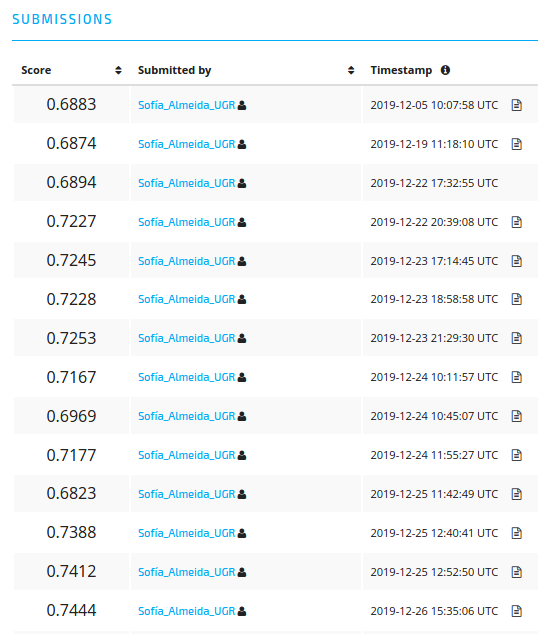
\includegraphics[height=1\textwidth, width=1\textwidth]{web1}
    \caption{Captura de pantalla de \textit{Submissions} - Parte 1.}
\end{figure}

\begin{figure}[H]
    \centering
    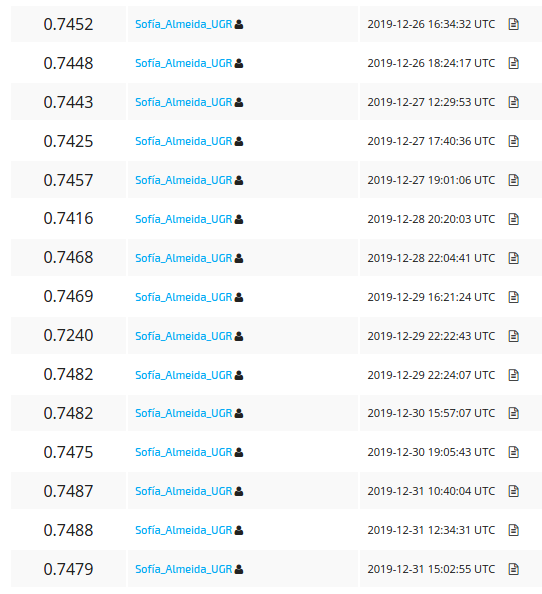
\includegraphics[height=1\textwidth, width=1\textwidth]{web2}
    \caption{Captura de pantalla de \textit{Submissions} - Parte 2.}
\end{figure}

\pagebreak

%% Índice
{\parskip=2pt
  \tableofcontents
}
\pagebreak

%%% Inicio del documento
%%%%%%%%%%%%%%%%%%%%%%%%%%%%%%%%%%%%%%%%%%%%%%%%%%%%%%%%%%%%%%%%%%%
%       Pruebas realizadas
%%%%%%%%%%%%%%%%%%%%%%%%%%%%%%%%%%%%%%%%%%%%%%%%%%%%%%%%%%%%%%%%%%%
\section{Pruebas realizadas}
\setlength\LTleft{-0.5in}
\setlength\LTright{-0.5in}
\begin{longtable}{lL{2.1cm}lllL{3cm}L{2.4cm}L{3.5cm}}
\caption{Pruebas realizadas}
\label{tab:pruebas}\\
\toprule
ID & Fecha-hora & Pos. & Sc.-Training & Sc.-Test & Preprocesado & Algoritmos & Parámetros\\
\midrule
00 & 5/12/2019 10:07:58 UTC & 315 & 0.7264 & 0.6883 &  & \textit{Lightgbm} & {\ttfamily objective = 'regression\_l1', n\_estimators = 200, n\_jobs = 2}\\
\arrayrulecolor{black!10}\midrule

01 & 19/12/2019 11:18:10 UTC & 356 & 0.7358 & 0.6874 &  & \textit{Lightgbm} & {\ttfamily objective = 'regression\_l1', n\_estimators = 200, n\_jobs = 2, feature\_fraction = 0.5, learning\_rate = 0.1, num\_leaves = 50}\\
\arrayrulecolor{black!10}\midrule

02 & 22/12/2019 17:32:55 UTC & 360 & 0.7294 & 0.6894 &  & \textit{Lightgbm} & {\ttfamily objective = 'regression\_l1', n\_estimators = 200, n\_jobs = 2, num\_leaves = 35, scale\_pos\_weight = 0.1}\\
\arrayrulecolor{black!10}\midrule

03 & 22/12/2019 20:39:08 UTC & 243 & 0.7339 & 0.7227 & \texttt{get\_dummies} para todas las variables categóricas & \textit{Lightgbm} & {\ttfamily objective = 'regression\_l1', n\_estimators = 200, n\_jobs = 2, num\_leaves = 40, scale\_pos\_weight = 0.1}\\
\arrayrulecolor{black!10}\midrule

04 & 23/12/2019 17:14:45 UTC & 242 & 0.7342 & 0.7245 & \texttt{get\_dummies} para todas las variables categóricas. Selección de variables con \texttt{VarianceThreshold}, umbral 0.95 & \textit{Lightgbm} & {\ttfamily objective = 'regression\_l1', n\_estimators = 200, n\_jobs = 2, num\_leaves = 40, scale\_pos\_weight = 0.1}\\
\arrayrulecolor{black!10}\midrule

05 & 23/12/2019 18:58:58 UTC & 242 & 0.7335 & 0.7228 & \texttt{get\_dummies} para todas las variables categóricas. Selección de variables con \texttt{SelectKBest}, $k =35$ & \textit{Lightgbm} & {\ttfamily objective = 'regression\_l1', n\_estimators = 200, n\_jobs = 2, num\_leaves = 40, scale\_pos\_weight = 0.1}\\
\arrayrulecolor{black!10}\midrule

06 & 23/12/2019 21:29:30 UTC & 234 & 0.7375 & 0.7253 & \texttt{get\_dummies} para todas las variables categóricas. Selección de variables con \texttt{VarianceThreshold}, umbral 0.95 & \textit{Lightgbm} & {\ttfamily objective = 'regression\_l1', n\_estimators = 200, n\_jobs = 2, num\_leaves = 45, scale\_pos\_weight = 0.1}\\
\arrayrulecolor{black!10}\midrule

07 & 24/12/2019 10:11:57 UTC & 237 & 0.8486 & 0.7167 & \texttt{get\_dummies} para todas las variables categóricas. Selección de variables con \texttt{VarianceThreshold}, umbral 0.9 & \textit{RandomForest} & {\ttfamily n\_jobs = -1, max\_depth = 20, n\_estimators = 300}\\
\arrayrulecolor{black!10}\midrule

08 & 24/12/2019 10:45:07 UTC & 237 & 0.8468 & 0.6969 & \texttt{get\_dummies} para todas las variables categóricas. Selección de variables con \texttt{VarianceThreshold}, umbral 0.9 & \textit{RandomForest} & {\ttfamily class\_weight = 'balanced', max\_depth = 20, max\_features = 'sqrt', n\_estimators = 300}\\
\arrayrulecolor{black!10}\midrule

09 & 24/12/2019 11:55:27 UTC & 237 & 0.9825 & 0.7177 & \texttt{get\_dummies} para todas las variables categóricas. Selección de variables con \texttt{VarianceThreshold}, umbral 0.95 & \textit{RandomForest} & {\ttfamily max\_depth = 40, max\_features = 'sqrt', n\_estimators = 500}\\
\arrayrulecolor{black!10}\midrule

10 & 25/12/2019 11:42:49 UTC & 239 & 0.7375 & 0.6823 & \texttt{OneHotencoder} para todas las variables categóricas. Selección de variables con \texttt{VarianceThreshold}, umbral 0.95 & \textit{Lightgbm} & {\ttfamily objective = 'regression\_l1', n\_estimators = 200, n\_jobs = 2, num\_leaves = 45, scale\_pos\_weight = 0.1}\\
\arrayrulecolor{black!10}\midrule

11 & 25/12/2019 12:40:41 UTC & 160 & 0.7693 & 0.7388 & \texttt{get\_dummies} para todas las variables categóricas. Selección de variables con \texttt{VarianceThreshold}, umbral 0.95 & \textit{Lightgbm} & {\ttfamily objective = 'regression\_l1', n\_estimators = 500, n\_jobs = -1, num\_leaves = 55, scale\_pos\_weight = 0.1}\\
\arrayrulecolor{black!10}\midrule

12 & 25/12/2019 12:52:50 UTC & 148 & 0.7855 & 0.7412 & \texttt{get\_dummies} para todas las variables categóricas. Selección de variables con \texttt{VarianceThreshold}, umbral 0.95 & \textit{Lightgbm} & {\ttfamily objective = 'regression\_l1', n\_estimators = 700, n\_jobs = -1, num\_leaves = 60, scale\_pos\_weight = 0.1}\\
\arrayrulecolor{black!10}\midrule

13 & 26/12/2019 15:35:06 UTC & 117 & 0.8070 & 0.7444 & \texttt{get\_dummies} para todas las variables categóricas. Selección de variables con \texttt{VarianceThreshold}, umbral 0.95 & \textit{Lightgbm} & {\ttfamily objective = 'regression\_l1', n\_estimators = 1000, n\_jobs = -1, num\_leaves = 65, scale\_pos\_weight = 0.1}\\
\arrayrulecolor{black!10}\midrule

14 & 26/12/2019 16:34:32 UTC & 107 & 0.8184 & 0.7452 & \texttt{get\_dummies} para todas las variables categóricas. Selección de variables con \texttt{VarianceThreshold}, umbral 0.95 & \textit{Lightgbm} & {\ttfamily objective = 'regression\_l1', n\_estimators = 1000, n\_jobs = -1, num\_leaves = 80, scale\_pos\_weight = 0.05}\\
\arrayrulecolor{black!10}\midrule

15 & 26/12/2019 18:24:17 UTC & 107 & 0.8259 & 0.7448 &\texttt{get\_dummies} para todas las variables categóricas. Selección de variables con \texttt{VarianceThreshold}, umbral 0.95 & \textit{Lightgbm} & {\ttfamily objective = 'regression\_l1', n\_estimators = 1000, n\_jobs = -1, num\_leaves = 90, scale\_pos\_weight = 0.05}\\
\arrayrulecolor{black!10}\midrule

16 & 27/12/2019 12:29:53 UTC & 110 & 0.8061 & 0.7443 & \texttt{get\_dummies} para todas las variables categóricas. Selección de variables con \texttt{VarianceThreshold}, umbral 0.95 & \textit{Lightgbm} & {\ttfamily objective = 'regression\_l1', n\_estimators = 900, n\_jobs = -1, num\_leaves = 70, scale\_pos\_weight = 0.05}\\
\arrayrulecolor{black!10}\midrule

17 & 27/12/2019 17:40:36 UTC & 110 & 0.7913 & 0.7425  & \texttt{get\_dummies} para todas las variables categóricas. Selección de variables con \texttt{VarianceThreshold}, umbral 0.95 & \textit{XGBoost} & {\ttfamily predictor = 'cpu\_predictor', n\_gpus = 0, n\_estimators = 200, eta = 0.3, max\_depth = 6, max\_delta\_step = 7}\\
\arrayrulecolor{black!10}\midrule

18 & 27/12/2019 19:01:06 UTC & 98 & 0.8691 & 0.7457 & \texttt{get\_dummies} para todas las variables categóricas. Selección de variables con \texttt{VarianceThreshold}, umbral 0.95 & \textit{XGBoost} & {\ttfamily n\_estimators = 700, eta = 0.1, max\_depth = 10}\\
\arrayrulecolor{black!10}\midrule

19 & 28/12/2019 20:20:03 UTC & 104 & 0.7862 & 0.7416 & \texttt{get\_dummies} para todas las variables categóricas. Selección de variables con \texttt{VarianceThreshold}, umbral 0.95 & StackingClassifier (\textit{Lightgbm}, \textit{RandomForest}, \textit{XGBoost}) & \textit{Lightgbm}: {\ttfamily objective = 'regression\_l1', n\_estimators = 700, n\_jobs = -1, num\_leaves = 65, scale\_pos\_weight = 0.05}. \textit{RandomForest}: {\ttfamily n\_jobs = -1, random\_state = 123456, max\_depth = 20, n\_estimators = 200}. \textit{XGBoost}: {\ttfamily n\_estimators = 400, eta = 0.1, max\_depth = 6}\\
\arrayrulecolor{black!10}\midrule

20 & 28/12/2019 22:04:41 UTC & 91 & 0.8436 & 0.7468 & \texttt{get\_dummies} para todas las variables categóricas. Selección de variables con \texttt{VarianceThreshold}, umbral 0.95 & StackingClassifier (\textit{Lightgbm}, \textit{XGBoost}) & \textit{Lightgbm}: {\ttfamily objective = 'regression\_l1', n\_estimators = 1000, n\_jobs = -1, num\_leaves = 80, scale\_pos\_weight = 0.05}. \textit{XGBoost}: {\ttfamily n\_estimators = 700, eta = 0.1, max\_depth = 10}\\
\arrayrulecolor{black!10}\midrule

21 & 29/12/2019 16:21:24 UTC & 92 & 0.8427 & 0.7469 & \texttt{get\_dummies} para todas las variables categóricas. Selección de variables con \texttt{VarianceThreshold}, umbral 0.95 & StackingClassifier (\textit{Lightgbm}, \textit{RandomForest}, \textit{XGBoost}) & \textit{Lightgbm}: {\ttfamily objective = 'regression\_l1', n\_estimators = 1000, num\_leaves = 80, scale\_pos\_weight = 0.05}. \textit{RandomForest}: {\ttfamily random\_state = 123456, max\_depth = 20, n\_estimators = 300}. \textit{XGBoost}: {\ttfamily n\_estimators = 700, eta = 0.1, max\_depth = 10}\\
\arrayrulecolor{black!10}\midrule

22 & 29/12/2019 22:22:43 UTC & 93 & 0.7387 & 0.7240 & \texttt{get\_dummies} para todas las variables categóricas. \texttt{Isolation Forest} con \texttt{outliers\_fraction = 0.05} para eliminar anomalías & \textit{Lightgbm} & {\ttfamily objective = 'regression\_l1', n\_estimators = 200, n\_jobs = 2, num\_leaves = 45, scale\_pos\_weight = 0.1}\\
\arrayrulecolor{black!10}\midrule

23 & 29/12/2019 22:24:07 UTC & 58 & 0.8421 & 0.7482 & \texttt{get\_dummies} para todas las variables categóricas & StackingClassifier (\textit{Lightgbm}, \textit{XGBoost}) & \textit{Lightgbm}: {\ttfamily objective = 'regression\_l1', n\_estimators = 1000, n\_jobs = -1, num\_leaves = 80, scale\_pos\_weight = 0.05}. \textit{XGBoost}: {\ttfamily n\_estimators = 700, eta = 0.1, max\_depth = 10}\\
\arrayrulecolor{black!10}\midrule

24 & 30/12/2019 15:57:07 UTC & 60 & 0.8498 & 0.7482 & \texttt{get\_dummies} para todas las variables categóricas & StackingClassifier (\textit{Lightgbm}, \textit{RandomForest}, \textit{XGBoost}) & \textit{Lightgbm}: {\ttfamily objective = 'regression\_l1', n\_estimators = 1000, num\_leaves = 80, scale\_pos\_weight = 0.05}. \textit{RandomForest}: {\ttfamily random\_state = 123456, max\_depth = 30, n\_estimators = 400}. \textit{XGBoost}: {\ttfamily n\_estimators = 700, eta = 0.1, max\_depth = 10}\\
\arrayrulecolor{black!10}\midrule

25 & 30/12/2019 19:05:43 UTC & 66 & 0.8604 & 0.7475 & \texttt{get\_dummies} para todas las variables categóricas & StackingClassifier (\textit{Lightgbm}, \textit{XGBoost}) & \textit{Lightgbm}: {\ttfamily objective = 'regression\_l1', n\_estimators = 1000, n\_jobs = -1, num\_leaves = 90, scale\_pos\_weight = 0.05}. \textit{XGBoost}: {\ttfamily n\_estimators = 900, eta = 0.1, max\_depth = 15}\\
\arrayrulecolor{black!10}\midrule

26 & 31/12/2019 10:40:04 UTC & 51 & 0.8627 & 0.7487 & \texttt{get\_dummies} para todas las variables categóricas & StackingClassifier (\textit{Lightgbm}, \textit{RandomForest}, \textit{XGBoost}) & \textit{Lightgbm}: {\ttfamily objective = 'regression\_l1', n\_estimators = 1000, num\_leaves = 80, scale\_pos\_weight = 0.05}. \textit{RandomForest}: {\ttfamily random\_state = 123456, max\_depth = 50, n\_estimators = 400}. \textit{XGBoost}: {\ttfamily n\_estimators = 700, eta = 0.1, max\_depth = 10}\\
\arrayrulecolor{black!10}\midrule
\rowcolor{SkyBlue}
27 & 31/12/2019 12:34:31 UTC & 51 & 0.8653 & 0.7488 & \texttt{get\_dummies} para todas las variables categóricas & StackingClassifier (\textit{Lightgbm}, \textit{RandomForest}, \textit{XGBoost}) & \textit{Lightgbm}: {\ttfamily objective = 'regression\_l1', n\_estimators = 1000, num\_leaves = 80, scale\_pos\_weight = 0.05}. \textit{RandomForest}: {\ttfamily random\_state = 123456, max\_depth = 60, n\_estimators = 450}. \textit{XGBoost}: {\ttfamily n\_estimators = 800, eta = 0.1, max\_depth = 10}\\
\arrayrulecolor{black!10}\midrule

28 & 31/12/2019 15:02:55 UTC & 51 & 0.8720 & 0.7479 & \texttt{get\_dummies} para todas las variables categóricas & StackingClassifier (\textit{Lightgbm}, \textit{RandomForest}, \textit{XGBoost}) & \textit{Lightgbm}: {\ttfamily objective = 'regression\_l1', n\_estimators = 1000, num\_leaves = 80, scale\_pos\_weight = 0.05}. \textit{RandomForest}: {\ttfamily random\_state = 123456, max\_depth = 65, n\_estimators = 500}. \textit{XGBoost}: {\ttfamily n\_estimators = 850, eta = 0.1, max\_depth = 12}\\
\arrayrulecolor{black}
\bottomrule
\end{longtable}

\begin{figure}[H]
  \makebox[\textwidth][c]{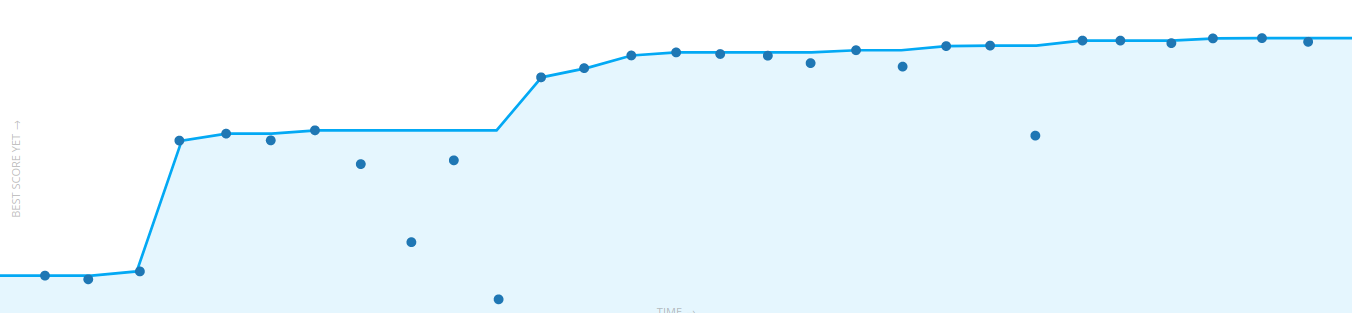
\includegraphics[height=0.65\textwidth, width=1.2\textwidth]{graph}}
    \caption{Gráfica de los \textit{submission} de la plataforma DrivenData.}
\end{figure}

\newpage

\section{Diario de pruebas}
\subsection{\texttt{p3\_00} - Archivo inicial}
Comenzamos aprendiendo a subir los resultados de \textit{test} a la plataforma para que puedan ser validados. El \textit{script} utilizado en esta ocasión es el proporcionado por el profesor de la asignatura. No se realiza ningún preprocesado y el algoritmo a utilizar es \textit{Lightgbm}. Este es un algoritmo de \textit{boosting} que se caracteriza por ser bastante rápido.

\subsection{Análisis exploratorio de los datos}

Antes de decidir qué hacer a continuación debemos conocer cierta información sobre los datos con los que estamos tratando. Pensamos que seguramente necesitemos algún tipo de preprocesado, pues es lo habitual en este tipo de problema, pero sin conocer exactamente cómo son los datos, si tienen o no ruido, la cantidad de valores perdidos, correlación entre las variables, \dots no podremos decidir cómo enfocar el preprocesado ni qué alternativas podrían venir bien al conjunto. Para ello comenzamos a escribir algunas funciones de visualización que nos permitan conocer esta información, se encuentran en el \textit{script} \texttt{visualization.py}.

Inspirándonos en \cite{noauthor_starter:_nodate}, observamos en la Figura \ref{fig:tam_clases} la distribución de las clases.

\begin{figure}[H]
    \centering
    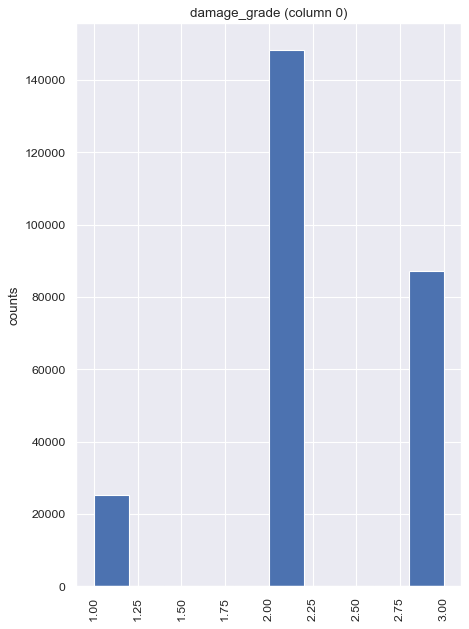
\includegraphics[height=0.6\textwidth, width=0.6\textwidth]{260601_dist}
    \caption{Tamaño de las clases.}
    \label{fig:tam_clases}
\end{figure}

Las clases del problema a tratar están claramente desbalanceadas. En la Tabla \ref{tab:tam_clas} observamos con exactitud el número de ejemplos que tenemos de cada clase. Ante esta situación se nos ocurren dos opciones: elegir un algoritmo que esté diseñado para manejar clases no balanceadas o utilizar técnicas específicas para paliar el desbalanceo.

% Tabla tamaño de clases
\begin{table}[H]
\centering
\caption{Tamaño de las clases.}
\label{tab:tam_clas}
\begin{tabular}{lrr}
\toprule
Clase & Número de elementos & Tamaño de la clase\\
\midrule
1 & 25124 & 9.64\%\\
2 & 148259 & 56.89\%\\
3 & 87218 & 33.47\%\\
\bottomrule
\end{tabular}
\end{table}

También podemos observar la correlación entre las variables en la Figura \ref{fig:corr_matrix}. No hay parejas de variables altamente correladas.

\begin{figure}[H]
  \centering
  \includesvg[height=1\textwidth, width=1\textwidth]{corr_matrix}
  \caption{Matriz de correlación.}
  \label{fig:corr_matrix}
\end{figure}

Continuamos el análisis tomando como referencia \cite{noauthor_model_nodate}. Mediante \texttt{data\_x.info()} vemos que de las 38 variables 30 son numéricas y 8 categóricas, accedemos a la descripción del problema en \cite{drivendata_richters_nodate-1}
para conocer cuántos posibles valores toman las variables categóricas. Tienen entre 3 y 10 posibles valores. En esta página también nos percatamos de que, de las variables numéricas, muchas son de tipo binario.

Ejecutando \texttt{data\_x.isnull().any()} nos damos cuenta de que nuestras variables no contienen valores perdidos, nos ahorraremos la imputación de valores perdidos.

\subsection{\texttt{p3\_01} - Ajuste de \textit{Lightgbm}}

Para tratar de conseguir mejores resultados tenemos, a priori, dos caminos: preprocesar los datos o mejorar el algoritmo. Para mejorar el algoritmo hay, a su vez, que tomar dos decisiones: elección del algoritmo y ajuste de sus parámetros.

En primer lugar, trataremos de ajustar los parámetros de \textit{Lightgbm} a ver si mejora el resultado. Usando el código de muestra \texttt{ejemplo\_ds\_avanzado.py}, implementamos \texttt{p3\_01.py}, donde nos centraremos en los parámetros \texttt{feature\_fraction} (que tomará valores entre 0.3 y 0.5), \texttt{learning\_rate} (probaremos 0.05 y 0.1) y \texttt{num\_leaves} (comprobaremos los valores 30 y 50), fijando \texttt{n\_estimators = 200}. Tras realizar el \texttt{GridSearch} se obtiene (tras 10 minutos de ejecución) que los mejores parámetros son: \texttt{feature\_fraction = 0.5}, \texttt{learning\_rate = 0.1},  \texttt{n\_estimators = 200}, \texttt{num\_leaves = 50}.

Obtenemos un resultado en \textit{training} de 0.7358 y en \textit{test} de 0.6874, disminuyendo con respecto al anterior envío, a pesar de haber aumentado en \textit{test}. ¿Se está produciendo sobreajuste?

\subsection{\texttt{p3\_02} - Parámetros de \textit{Lightgbm} contra el desbalanceo}

%% Comprobamos qué ocurre si nos quedamos con menor \texttt{learning\_rate}. Usamos los parámetros ajustados, modificando solo la variable comentada. Los parámetros utilizados son: \texttt{feature\_fraction = 0.5}, \texttt{learning\_rate = 0.05},  \texttt{n\_estimators = 200}, \texttt{num\_leaves = 50}.
Nos preguntamos qué está provocando este sobreajuste, así comprobamos los valores de las variables por defecto y los utilizados. El que más se diferencia es \texttt{num\_leaves}, por defecto es 31 y estamos tomando 50. Es complicado saber hasta qué punto podemos aumentar el número de hojas sin que se llegue a producir el sobreajuste que provoca malos resultados en la fase de \textit{test}, más teniendo en cuenta que el número de pruebas a realizar es limitado. Por ello, proseguiré tratando de mejorar el rendimiento de este algoritmo de otro modo.

% https://lightgbm.readthedocs.io/en/latest/Parameters.html
Leemos en \cite{noauthor_parameters_nodate} que \textit{Lightgbm} tiene dos parámetros que nos permiten tratar de ajustar el desbalanceo de las clases: \texttt{is\_unbalance} o \texttt{scale\_pos\_weight}.
Probaremos a configurar ambos parámetros a ver con cuál conseguimos mejor resultado.

En \texttt{p3\_02\_unbalance.py} partimos del código utilizado en \texttt{p3\_00.py} añadiendo las variables \texttt{num\_classes = 3} y \texttt{is\_unbalance = True}. Conseguimos exactamente el mismo resultado que en el archivo de partida (los archivos \texttt{submission} correspondientes no se diferencian) a pesar de que por defecto (en \texttt{p3\_00.py}) se asumía que no había desbalanceo. 

Probamos con la otra opción: variamos el peso de la clase positiva (asumimos que está tomando la mayoritaria como positiva) entre 0.1 y 0.6 modificando el parámetro \texttt{scale\_pos\_weight}.
Así, terminamos ejecutando el algoritmo con {\ttfamily n\_estimators = 200, num\_leaves = 35, scale\_pos\_weight = 0.1}, consiguiendo una puntuación de 0.7294 en entrenamiento y 0.6894 al realizar el envío (mejorando la mejor solución obtenida hasta el momento).

\subsection{\texttt{p3\_03} -  Binarización de variables categóricas}

% https://pandas.pydata.org/pandas-docs/stable/reference/api/pandas.get_dummies.html
Una opción que podemos utilizar para preprocesar es, en vez de convertir las variables categóricas a numéricas, realizar un \textit{one-to-many} en el que binarizamos las variables categóricas, obteniendo una variable nueva por cada posible valor de las variables categóricas. Como observamos que eran 8 variables categóricas y que no tomaban demasiados valores, además de que \textit{Lightgbm} es un algoritmo rápido, probamos este preprocesado. 

Pandas ofrece una función que realiza la transformación sobre el conjunto de datos, es la función \texttt{get\_dummies} \cite{noauthor_pandas.get_dummies_nodate}. En el archivo \texttt{p3\_03.py} encontramos el código correspondiente a esta ejecución. Pasamos de 38 a 68 características.

Conseguimos una puntuación en \textit{training} de 0.7339 y en \textit{test} de 0.7227 (mejorando los resultados anteriores).

\subsection{\texttt{p3\_04} - Selección de variables con \texttt{VarianceThreshold}}

Aunque \textit{Lightgbm} es un algoritmo ligero y se puede ejecutar con las 68 variables que conseguimos tras binarizar las categóricas, puede que no todas ellas sean importantes para clasificar si el edificio ha sido dañado o no, alejando el modelo del modelo ideal. Por ello, partiendo del código anterior en el que utlizamos \textit{Lightgbm} con 0.1 para \texttt{scale\_pos\_weight} añadimos un método de selección de variables al preprocesado. En \textit{scikit-learn} vienen implementados distintos métodos de selección de características \cite{noauthor_1.13._nodate}.

Nuestro primer intento consiste en eliminar las variables con varianza baja \cite{noauthor_sklearn.feature_selection.variancethreshold_nodate}. Por defecto, elimina las variables que tengan varianza nula, esto es, aquellas variables que tengan el mismo valor para todos los ejemplos. Indicamos un umbral para que elimine. Por ejemplo, para 0.9 obtenemos de \textit{f1-score} en \textit{training} 0.7319 (22 variables, en torno a 15 segundos por partición). Con un umbral de 0.95 nos quedamos con 33 variables finalmente, los tiempos por partición van desde 16 hasta 20 segundos, pero la puntuación se ve favorecida (en \textit{training}) siendo ahora 0.7342. La puntuación al subirlo en la web es de 0.7245 (mejorando en milésimas al programa base sin selección de variables).

%https://stackoverflow.com/questions/53413701/feature-importance-using-lightgbm/53578643#53578643
Tratamos de ver la importancia de cada variable mediante la función \texttt{plotImp} que generará un gráfica como la que podemos ver en la Figura \ref{fig:lgbm_imp_04}. En ella se representa el número de veces que una variable se usa en un modelo.
\begin{figure}[H]
     \makebox[\textwidth][c]{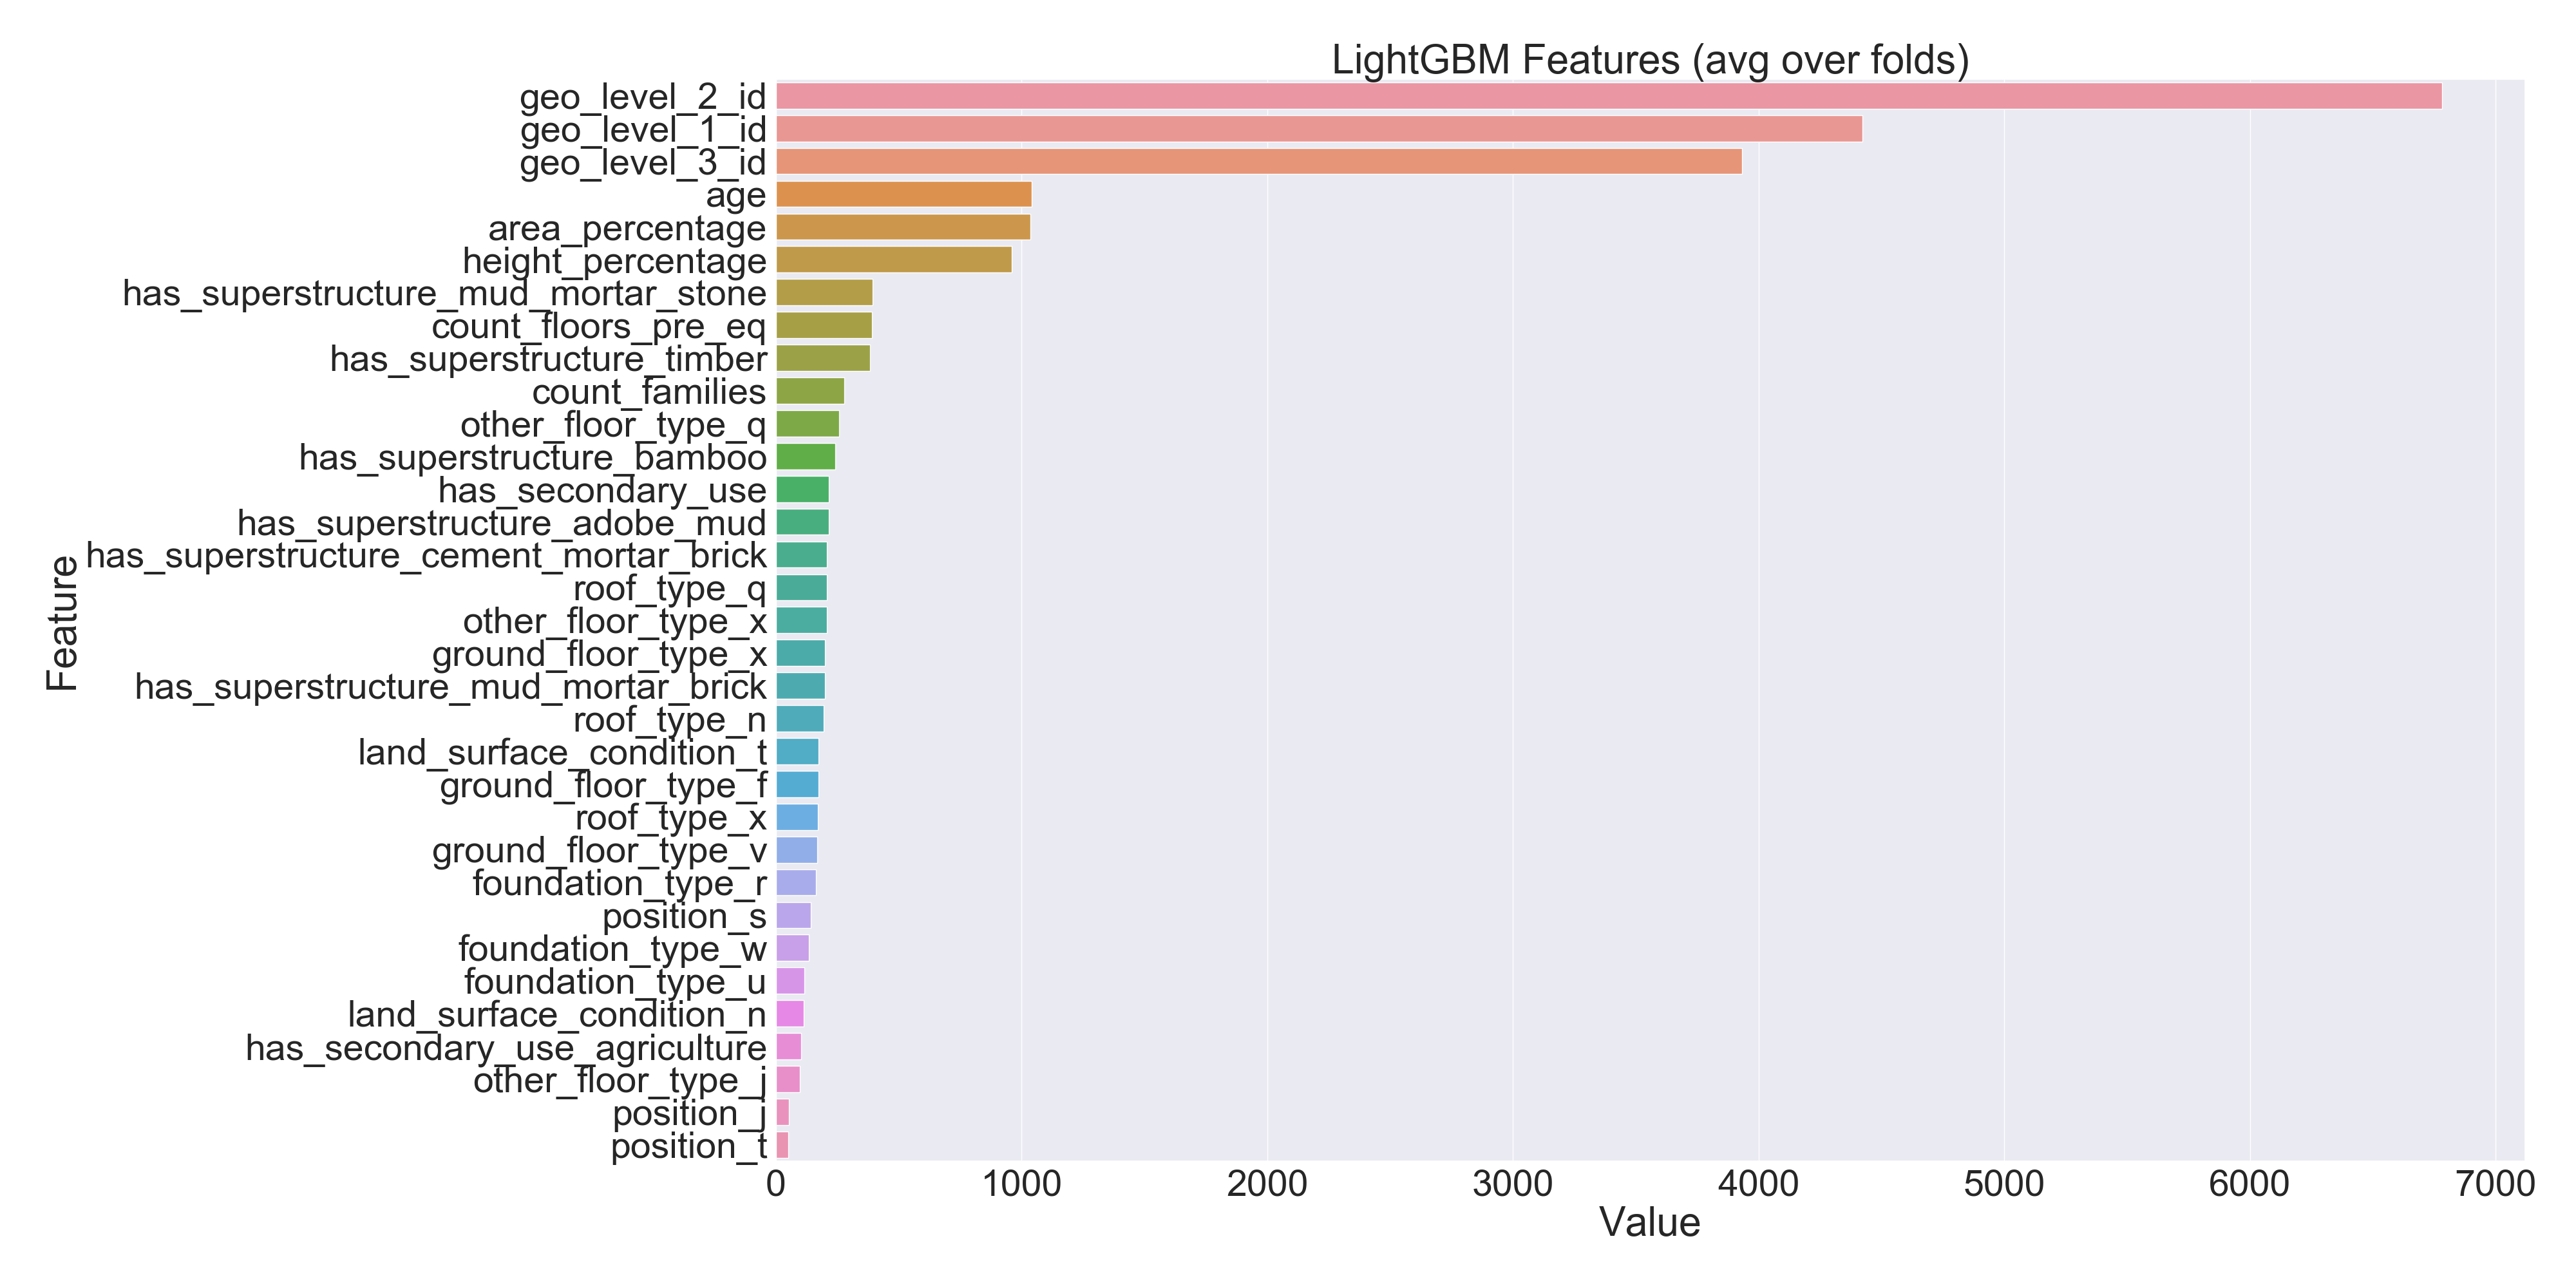
\includegraphics[height=0.8\textwidth, width=1.1\textwidth]{lgbm_importances04}}
    \caption{Importancia de las variables - \texttt{VarianceThreshold}, umbral = 0.95.}
    \label{fig:lgbm_imp_04}
\end{figure}

\subsection{\texttt{p3\_05} - Selección de variables con \texttt{SelectKBest}}
Seleccionando variables a partir de su varianza hemos mejorado algunas milésimas el resultado, igual utilizando algún otro método de selección más complejo logramos ajustarnos un poco mejor a las variables realmente determinantes en nuestro problema.

Probamos a seleccionar las $k$ mejores variables según \textit{tests} estadísticos univariantes \cite{noauthor_sklearn.feature_selection.selectkbest_nodate}.

Notamos que los tiempos de ejecución disminuyen, pasan a rondar los 10 segundos. El resultado en entrenamiento es una puntuación \textit{f1-score} de 0.7251 para 10 características. Observamos en la Figura \ref{fig:lgbm_imp_05_10} que las cuatro primeras variables son las mismas que seleccionando según la varianza, pero a partir de ahí varían.

\begin{figure}[H]
    \centering
     \makebox[\textwidth][c]{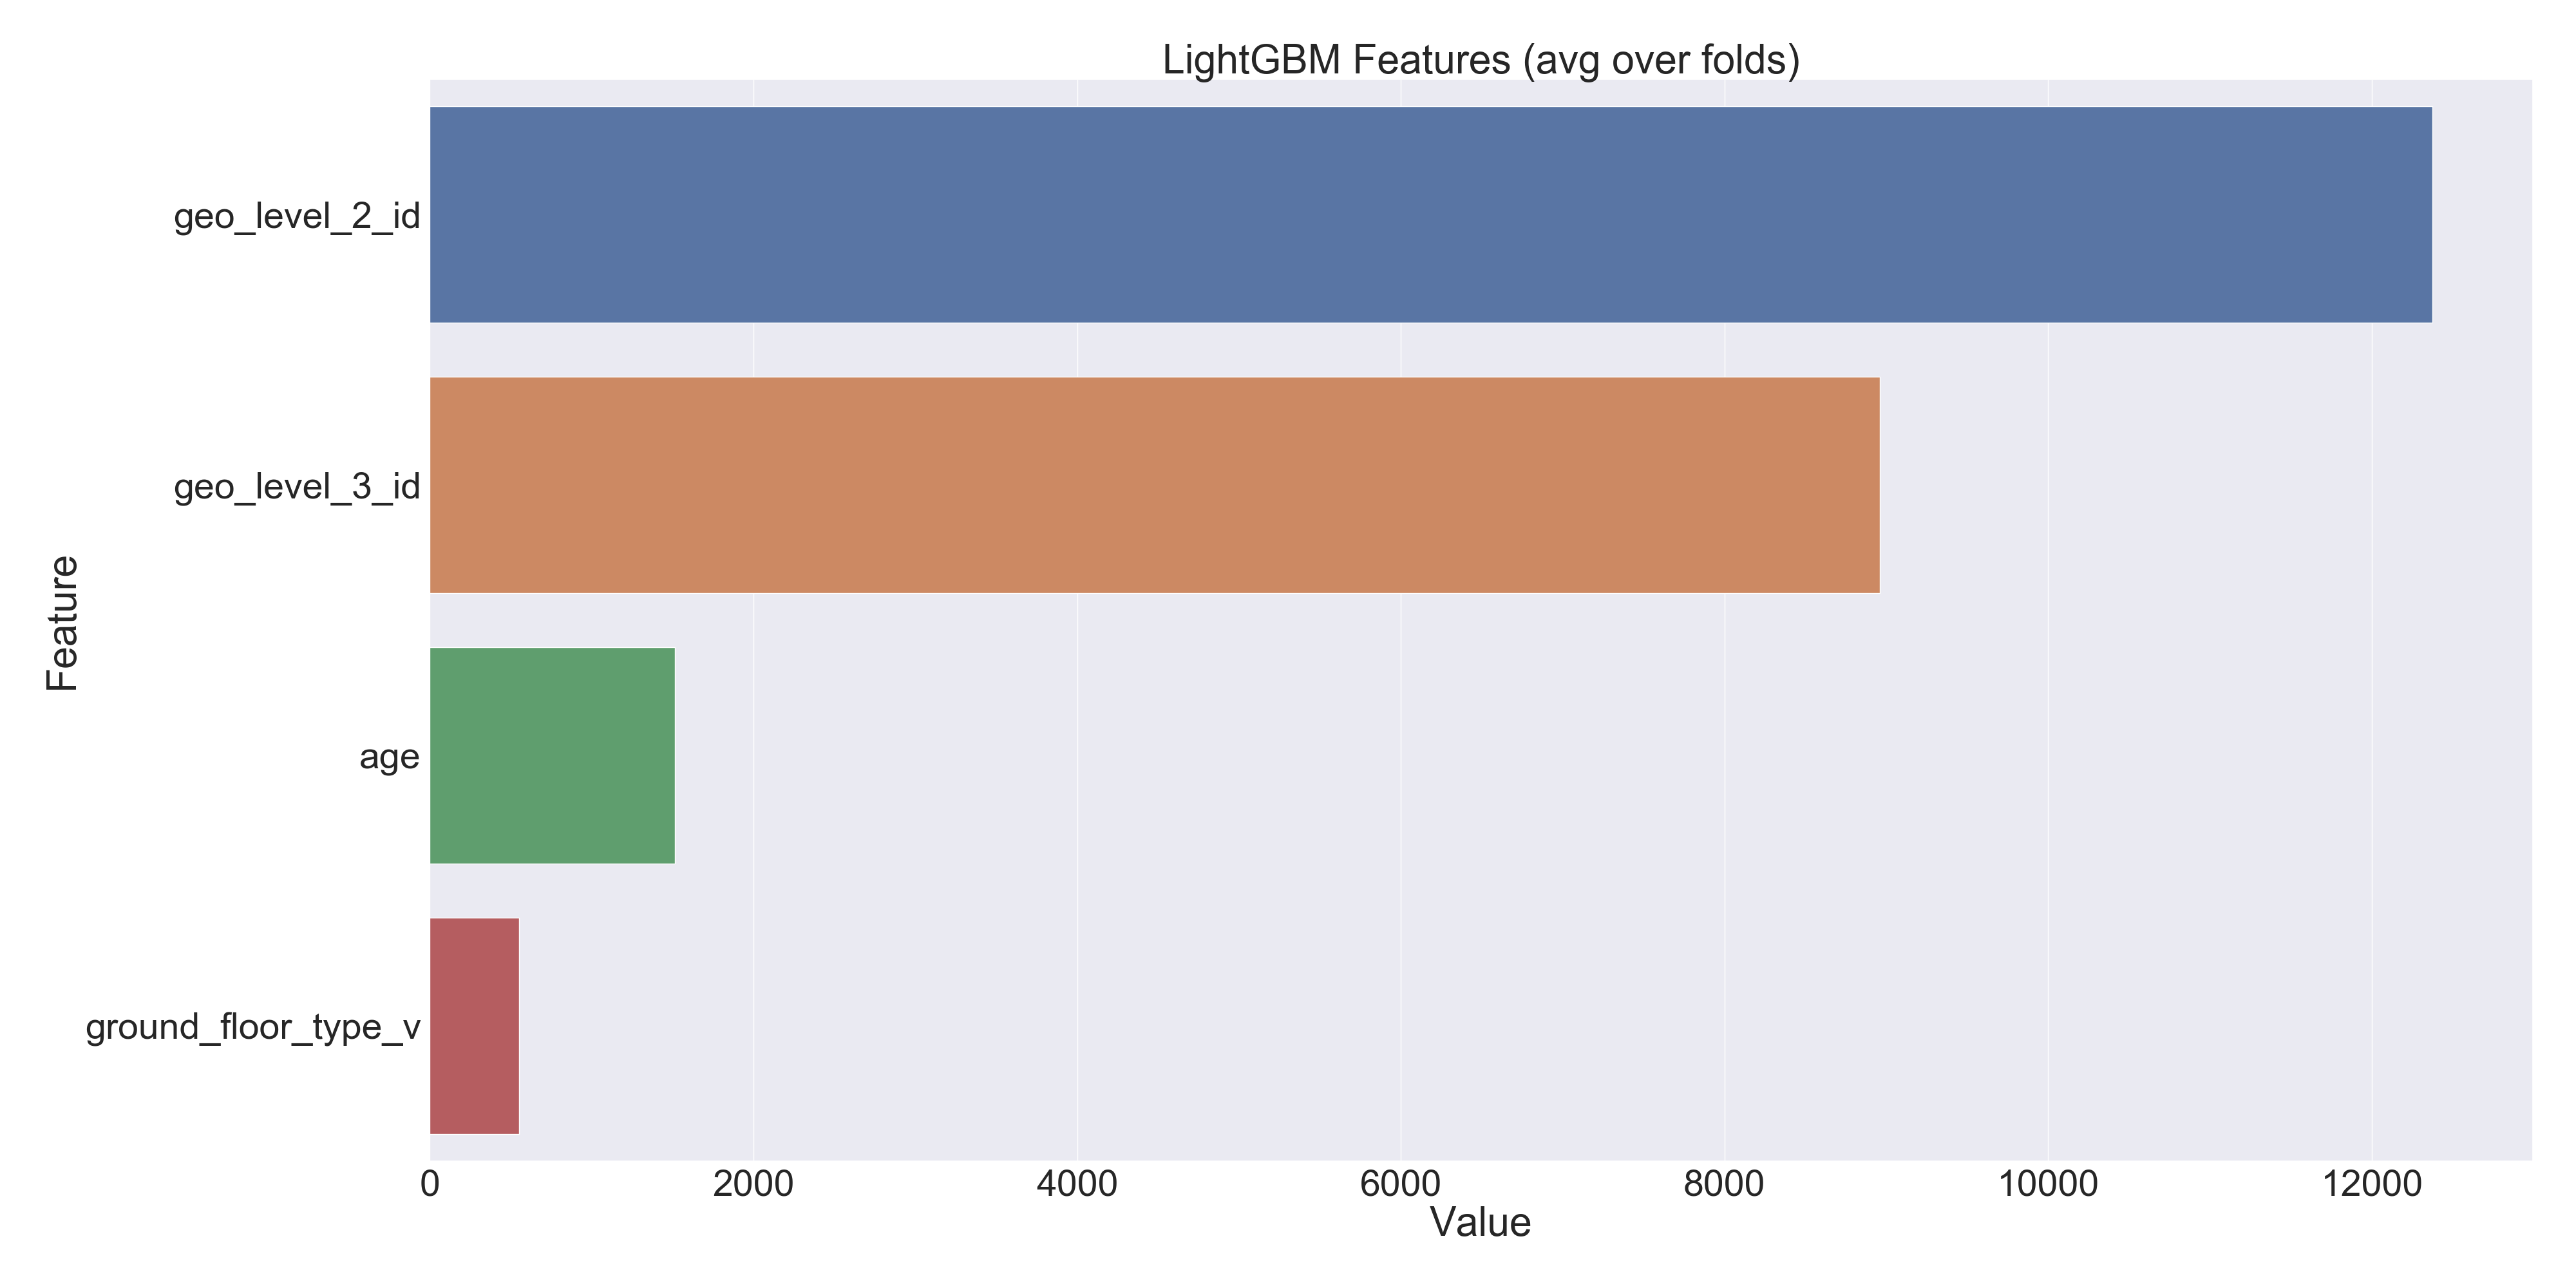
\includegraphics[height=0.9\textwidth, width=1.2\textwidth]{lgbm_importances_05_10}}
    \caption{Importancia de las variables tras seleccionar las 10 mejores - \texttt{SelectKBest}.}
    \label{fig:lgbm_imp_05_10}
\end{figure}

Si nos quedamos solo con 4 variables no selecciona estas cuatro (se queda con \texttt{geo\_level\_2\_id, geo\_level\_3\_id, age} y \texttt{ground\_floor\_type\_v}) y el rendimiento baja a 0.6772.

Como no sabemos cuál es la mejor forma de seleccionar el valor $k$ del preprocesado realizamos pruebas con algunos valores para elegir el mejor. En la Tabla \ref{tab:05_k} podemos ver los diferentes valores probados.

\begin{table}[H]
\centering
\caption{Selección de las $k$ mejores características.}
\label{tab:05_k}
\begin{tabular}{lrr}
\toprule
Nº de variables & F1-Score & Tiempo por partición ($s$)\\
\midrule
4 & 0.6772 & ~7\\
10 & 0.7251 & 9.5 - 13\\
20 & 0.7296 & 10 - 15\\
25 & 0.7317 & 12 - 17\\
30 & 0.7325 & 17 - 18\\
35 & 0.7335 & 18 - 20\\
37 & 0.7294 & 19 - 21\\
40 & 0.7302 & 18 - 23\\
\bottomrule
\end{tabular}
\end{table}

Nos quedamos con 35 variables consiguiendo una puntuación en \textit{test} de 0.7228 (parecida a la conseguida sin realizar la selección de variables). En la Figura \ref{fig:lgbm_imp_05_35} observamos las variables más utilizadas para clasificar en esta ocasión.

\begin{figure}[H]
    \centering
    \makebox[\textwidth][c]{\includegraphics[height=0.9\textwidth, width=1.2\textwidth]{lgbm_importances_05_35}}
    \caption{Importancia de las variables tras seleccionar las 35 mejores.}
    \label{fig:lgbm_imp_05_35}
\end{figure}

Comparando con las seleccionadas en p3\_04 nos damos cuenta de que aunque las primeras son similares y coinciden en algunas más, \texttt{height\_percentage} es de las más utilizadas en el caso anterior y en este no fue seleccionada.

\subsection{\texttt{p3\_06} - Variación de los parámetros de \textit{Lightgbm}}
Tras perder el rato con algunas pruebas fallidas, decidimos no desperdiciar la última subida del día. Utilizaremos \texttt{get\_dummies} y \texttt{VarianceThreshold} en el preprocesado y el algoritmo \textit{Lightgbm} aumentando el número de hojas a 45. La puntuación en \textit{training} es de 0.7375 y en \textit{test} de 0.7253 (mejor hasta el momento).

\subsection{\texttt{p3\_07} - \textit{RandomForest}}

Pasamos ahora a probar otro algoritmo: \textit{RandomForest} \cite{noauthor_3.2.4.3.1._nodate}.

Investigando un poco vemos que aunque en teoría los árboles de decisión puedan trabajar con todo tipo de variables, en la práctica la implementación de los algoritmos no lo permite. Así que en este caso también debemos numerizar las variables categóricas.

Empezamos de forma similar a como lo hicimos con \textit{Lightgbm}. Numerizamos las variables categóricas, haciendo un preprocesado mínimo. Realizamos un ajuste de parámetros mínimo para ver qué variables puede ser más interesante afinar.

Como tarda mucho tiempo, decido probar las opciones que funcionaron mejor con \textit{Lightgbm}, a ver si en este caso también dan buenos resultados. Utilizando como criterio de selección la varianza e imponiendo un umbral de 0.9 nos quedamos con 22 variables que serán las utilizadas con \textit{RandomForest}. Tarda unos 8 minutos con el \texttt{GridSearch} en el que se probó \texttt{max\_depth: [10, 20]} y \texttt{n\_estimators:[200, 300]}. Los mejores parámetros resultan ser \texttt{max\_depth = 20} y \texttt{n\_estimators = 300}.
Con un tiempo de ejecución de más de un minuto por partición (en torno a los 70 segundos) consigue una puntuación en \textit{training} de 0.8486 y en \textit{test} de 0.7167.

\subsection{\texttt{p3\_08} - Ajuste de \textit{RandomForest}}

Para tratar de paliar el sobreaprendizaje, siguiendo la recomendación de \cite{noauthor_1.11._nodate} se fija el número máximo de características en la raíz cuadrada del número de características, confiando también que esto disminuya un poco el tiempo de cómputo. Además, se modifica la variable \texttt{class\_weight} con la que se actuará sobre el desbalanceo. Se consideran distintas opciones desde el balanceo automático calculado por el algoritmo hasta algunas combinaciones de pesos puestas manualmente. Tras realizar el ajuste de parámetros mediante \texttt{GridSearch} (que llevó unos 12 minutos), se elige la siguiente combinación de los mismos: {\ttfamily class\_weight = 'balanced', max\_depth = 20, max\_features = 'sqrt', n\_estimators = 300}.

Cada partición tarda unos 70 segundos. Se consigue una puntuación en entrenamiento de 0.8468 (menor que antes), confiando en que el sobreajuste sea menor lo subimos y obtenemos una puntuación de 0.6969 (¡peor que sin balancear!).

\subsection{\texttt{p3\_09} - Ajuste de \textit{RandomForest}}
Probamos a quitar \texttt{max\_features = 'sqrt'}, obtenemos una puntuación en \textit{training} de 0.8468 (igual que cuando sí que estaba).

Si lo mantenemos pero quitamos el \texttt{class\_weight='balanced'} la puntuación en entrenamiento es de 0.8486, así que decidimos quitar este parámetro pues sin él mejora un poco el resultado.

Por último, tratamos de mejorar un poco aumentando la profundidad máxima, número de estimadores y número de variables. Para ello, se toma en la selección de variables \texttt{threshold=(.95 * (1 - .95))}, \texttt{max\_depth = 40}, \texttt{n\_estimators = 500}, \texttt{max\_features = 'sqrt'}. Las iteraciones aumentan su tiempo de ejecución hasta superar los dos minutos (en torno a 150 segundos). La puntuación en entrenamiento es de 0.9825, ¿estará sobreajustando? Lo comprobamos subiendo los resultados y obteniendo una puntuación de 0.7177. ¿Cómo podemos evitar este sobreajuste?

\subsection{\texttt{p3\_10} - Binarización con \texttt{OneHotEncoder}}

El gran sobreajuste de \textit{RandomForest} y su tiempo elevado de ejecución hace que abandonemos este algoritmo de momento y volvamos a \textit{Lightgbm}.
A partir de \cite{noauthor_richters_nodate} descubrimos que \texttt{get\_dummies} no es la única forma de categorizar variables. Como este cambio hizo que mejoraran los resultados probamos diferentes formas de binarizar \cite{liu_encoding_2018} a ver si varían los resultados.

Partiendo del código \texttt{p3\_06.py} que fue el que mejores resultados dio, realizaremos la binarización con \texttt{OneHotEncoder}.
El resultado en \textit{training} es similar al del código original aunque si comparamos los archivos \textit{submission} correspondientes nos damos cuenta de que difieren en 10273/86867\footnote{Realizamos este cálculo mediante \texttt{diff -U 0 file1 file2 | grep \^{} @ | wc -l}.} objetos, probamos a subirlo a ver cuál es mejor. Sin embargo, el resultado en \textit{test} es bastante peor, de 0.6823\footnote{Aquí nos quedamos con la duda de si subimos el archivo correcto, esperábamos resultados similares al menos a los obtenidos con \texttt{get\_dummies}. La limitación en el número de envíos hizo que nunca lo comprobara.}.

\subsection{\texttt{p3\_11} - Binarización con \texttt{DictVectorizer}}

Volvemos a partir del código de \texttt{p3\_06.py} y probamos la otra alternativa de \cite{liu_encoding_2018}: \texttt{DictVectorizer} \cite{noauthor_sklearn.feature_extraction.dictvectorizer_nodate}.

Tras la binarización y selección de variables se consiguen otra vez 33 y una puntuación en \textit{training} de 0.7375, pero en este caso tenemos 0 diferencias con el original. Guardamos este código en el archivo \texttt{p3\_dict.py} y tratamos de ajustar un poco más los parámetros utilizados en \texttt{p3\_06.py}.

Así, probamos las combinaciones de los parámetros: \texttt{learning\_rate = 0.1}, \texttt{num\_leaves = [45, 50, 55]}, \texttt{n\_estimators = [200, 300, 400, 500]}.

Tras largo rato de ejecución para probar todas las combinaciones (36), se concluye que los mejores parámetros son: \texttt{num\_leaves = 55} y \texttt{n\_estimators = 500}. El aumento de estos valores provoca un incremento en el tiempo de ejecución (unos 40 segundos por partición). Consiguiendo un \textit{f1-score} en entrenamiento de 0.7693, que se traduce en un valor en \textit{test} de 0.7388 (mejor hasta el momento).

\subsection{\texttt{p3\_12} - Ajuste \textit{Lightgbm}}

Parece que aumentar el número de hojas y estimadores es positivo para el resultado, pruebo a ejecutar una variación del archivo \texttt{p3\_11}, esta vez con \texttt{num\_leaves = 60} y \texttt{n\_estimators = 700}. El tiempo de ejecución se ve afectado, cada partición tarda entre 50 y 60 segundos. Consigo una puntuación en \textit{training} de 0.7855 y en \textit{test} de 0.7412 (mejor que en el archivo de partida, reforzando la hipótesis).

\subsection{\texttt{p3\_13} - Ajuste \textit{Lightgbm}}

Nos preguntamos cuánto podemos aumentar estos valores antes de que se produzca sobreajuste. Ejecutamos, volviendo a aumentar ambos valores:  \texttt{num\_leaves = 65} y \texttt{n\_estimators = 1000}. Los tiempos de ejecución pasan a estar en el rango 60-75 segundos por partición. Conseguimos una puntuación al entrenar de 0.8070 y al realizar un envío de 0.7444, mejorando el resultado anterior.

\subsection{\texttt{p3\_14} - Ajuste \textit{Lightgbm}}

Podemos hacer pruebas para tratar de ajustar el resto de parámetros, para ello partimos del archivo \texttt{p3\_06.py} (para evitar tiempos de ejecución demasiado grandes) y asumiremos que si mejora en este caso, mejorará al aumentar el número de estimadores y hojas.

Pasamos a comprobar qué umbral es el más adecuado en la selección de variables, en la Tabla \ref{tab:14} podemos observar los resultados de las ejecuciones para el distinto valor del umbral.

\begin{table}[H]
\centering
\caption{Selección de características variando el umbral.}
\label{tab:14}
\begin{tabular}{lrrr}
\toprule
Umbral & Nº variables & F1-Score - Trainig & Tiempo por partición ($s$)\\
\midrule
0.9 & 22 & 0.7341 & 14-16\\
0.91 & 24 & 0.7344 & 14-17 \\
0.92 & 26 & 0.7348 & 15-19 \\
0.93 & 27 & 0.7356 & 16-22 \\  
0.94 & 30 & 0.7364 & 21-26 \\
%0.945 & 31 & 0.7375 & 16-19\\
0.95 & 33 & 0.7375 & 14-18\\
0.96 & 37 & 0.7372 & 17-20\\ 
\bottomrule
\end{tabular}
\end{table}

Parece que el umbral más adecuado es el que habíamos elegido, 0.95.

El siguiente parámetro a ajustar será \texttt{scale\_pos\_weight}, relativo al desbalanceo de las clases. Para ajustarlo utilizaremos un \texttt{GridSearch} en el que comprobaremos qué valor es mejor entre \texttt{[0.05, 0.075, 0.1, 0.15, 0.175]} (5 min para las pruebas, archivo \texttt{p3\_14\_sc.py}). El que mejor resultados da es 0.05, con un resultado en \textit{training} de 0.7375 (tiempo entre 19 y 25 segundos por partición), si lo comparamos con \texttt{p3\_06.py} es exactamente igual. ¿Será mejor si lo bajamos más?

Modificamos el archivo para probar valores menores \texttt{[0.05, 0.04, 0.03, 0.02, 0.01]}, el mejor parámetro sigue siendo 0.05.

Partiremos del archivo \texttt{p3\_13.py} con este parámetro ya ajustado y aumentando el número de hojas a 80. El tiempo de ejecución por partición es de 75 - 100 segundos. La puntuación en \textit{training} es 0.8184 y la puntuación en \textit{test} es de 0.7452 (mejorando levemente la de partida).

\subsection{\texttt{p3\_15} - Análisis sobre las variables \texttt{geo\_level\_i\_id}}

En nuestras gráficas de selección de características destacaba que las primeras variables coincidían en todas ellas, eran las llamadas \texttt{geo\_level\_i\_id}. Estas variables representan las regiones geográficas en las que están situadas los edificios.

Investigando un poco descubrimos que Nepal está fromado por 7 provincias, cada una de las cuales tiene una serie de distritos (entre 8 y 14), en total hay 77 distritos. La variable \texttt{geo\_level\_1\_id} toma valores entre 0 y 30, no logro saber bien a qué hace referencia.

En las Figuras \ref{fig:geo11} y \ref{fig:geo12} observamos la relación entre los valores que toma esta variable y el grado de daño del edificio, que resulta ser un poco dispar.

\begin{figure}[H]
    \centering
    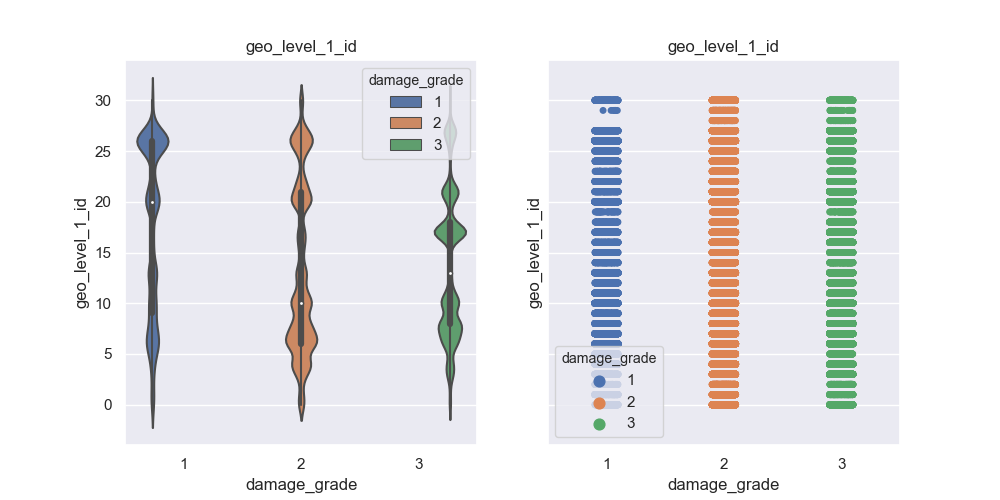
\includegraphics[height=0.8\textwidth, width=1.0\textwidth]{geo_level_1_1}
    \caption{Relación \texttt{geo\_level\_1\_id} y \texttt{damage\_grade}.}
    \label{fig:geo11}
\end{figure}

\begin{figure}[h]
    \centering
    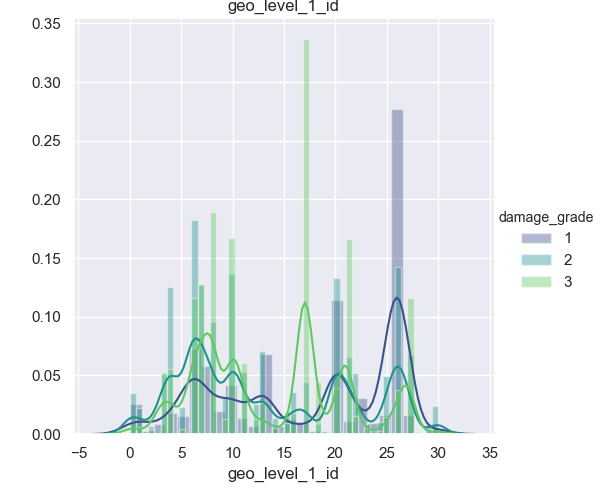
\includegraphics[height=0.8\textwidth, width=1.0\textwidth]{geo_level_1_2}
    \caption{Relación \texttt{geo\_level\_1\_id} y \texttt{damage\_grade}.}
    \label{fig:geo12}
\end{figure}

En cualquier caso, es una variable categórica que está tomando valores numéricos, es decir, se le está induciendo cierto orden que a priori no tienen. Podemos probar a binarizar esta variable a ver si los resultados mejoran. Si hiciéramos lo mismo con geo\_level\_2 y 3 aumentaría demasiado el número de variables, además, en esos casos la relación entre su valor y el grado de daño es uniforme, como podemos ver en las Figuras \ref{fig:geo21} y \ref{fig:geo31}.

\begin{figure}[H]
    \centering
    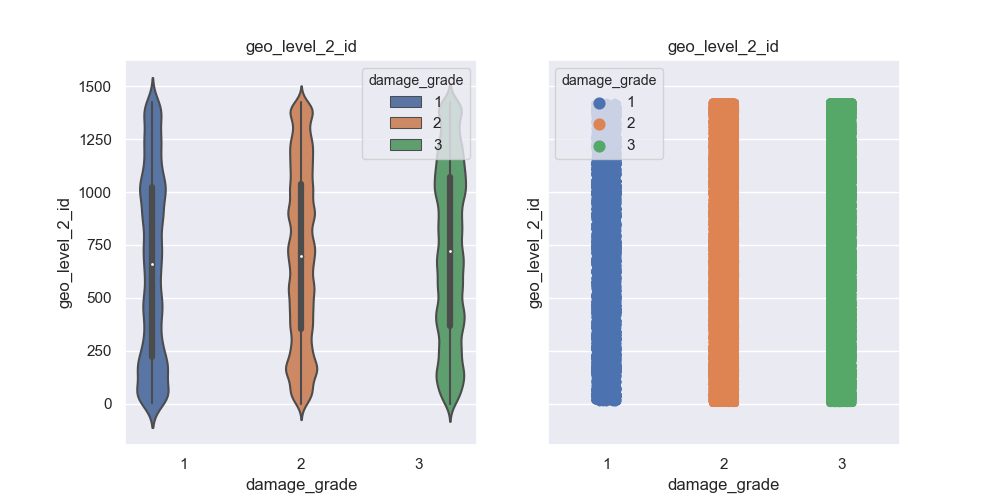
\includegraphics[height=0.8\textwidth, width=1.0\textwidth]{geo_level_2_1}
    \caption{Relación \texttt{geo\_level\_2\_id} y \texttt{damage\_grade}.}
    \label{fig:geo21}
\end{figure}

\begin{figure}[H]
    \centering
    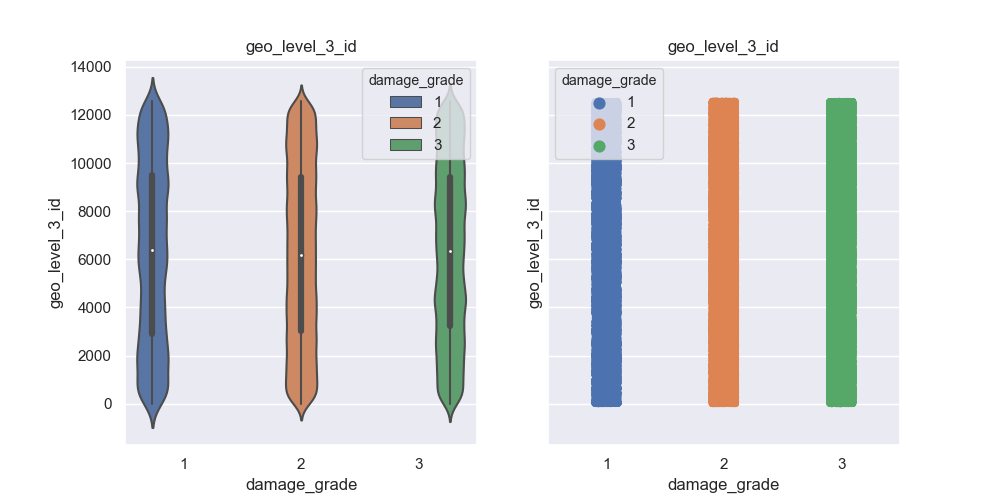
\includegraphics[height=0.8\textwidth, width=1.0\textwidth]{geo_level_3_1}
    \caption{Relación \texttt{geo\_level\_3\_id} y \texttt{damage\_grade}.}
    \label{fig:geo31}
\end{figure}

Tras binarizar \texttt{geo\_level\_1\_id} (además de las categóricas) tenemos 98 variables que al seleccionar se quedan en 41. Las pruebas iniciales se hacen partiendo de \texttt{p3\_06.py} por evitar tiempos de ejecución demasiado elevados. Conseguimos un resultado en \textit{training} de 0.7291, menor que el 0.7375 obtenido en el intento 06 con tiempos entre 17 y 22 segundos.

Probamos a realizar lo mismo, aumentando el umbral de selección a 0.97, en este caso nos quedamos con 52 variables, los tiempos de ejecución van de 18 segundos hasta 23. El resultado en \textit{training} es ahora de 0.7337 (sigue siendo inferior al de partida).

Un umbral de 0.99, nos deja con 70 variables y tiempos entre 20 y 24 segundos por partición. Siendo los resultados en entrenamiento otra vez inferiores a los de partida: 0.7369.
% error de discrepancia en número...

Si nos quedamos con las 98 variables los tiempos van desde 19 hasta 24 y el resultado es de 0.7361 (menor que en el caso anterior).

No conseguimos una mejora, con lo que concluimos que al numerizar igual sí que estaban ordenadas según algún criterio (situación, proximidad, ...).

Como no nos queda mucho más tiempo hoy, probamos a aumentar el número de hojas para tratar de mejorar el intento 14. Tarda unos 80 segundos por partición. El resultado en \textit{training} es de 0.8259 y en \textit{test} de 0.7448 (un poco peor que el intento 14 de partida). Debe de ser que se está produciendo sobreajuste.

\subsection{\texttt{p3\_16} - Ajuste de \textit{Lightgbm}}

Hemos visto que los parámetros \texttt{num\_leaves} y \texttt{n\_estimators} son determinantes para la buena ejecución del algoritmo \textit{Lightgbm}, por ello, realizaremos un ajuste de parámetros específico a ver qué combinación de parámetros proporciona mejores resultados. Probaremos los valores de los parámetros: \texttt{num\_leaves $\in$ \{50, 60, 70, 80, 90, 100\}, n\_estimators $\in$ \{200, 300, 400, 500, 600, 700, 800, 900, 1000\},
  scale\_pos\_weight $\in$ \{0.05, 0.1\}}. Tras  142.4 minutos de ejecución, se llega a la conclusión de que los mejores parámetros son: {\ttfamily n\_estimators = 900, num\_leaves = 70, scale\_pos\_weight = 0.05}. En torno a los 70 segundos de ejecución por partición, cosigue un resultado en entrenamiento de 0.8061.

Si probamos la binarización de geo\_level\_1\_id (\texttt{p3\_16\_geo.py}) con estos parámetros se queda con 41 variables, tiempo por partición entre 65 y 80 segundos. El resultado en \textit{training} es de 0.7995, un poco menor que sin la binarización.

Así, subimos los resultados de la ejecución sin binarizar esta variable obteniendo un resultado en \textit{test} de 0.7443 (menor que el obtenido en \texttt{p3\_14}). 

\subsection{\texttt{p3\_17} - \textit{XGBoost}}

Pasamos ahora a probar otro algoritmo. Sabemos que \textit{Lightgbm} tiene la ventaja de ser muy eficiente, pero no es el más potente, así, probaremos con \textit{XGBoost} \cite{noauthor_xgboost_nodate}, a ver si obtiene resultados similares o incluso mejores. Utilizaremos el preprocesado anterior.

En primer lugar, nos encontramos con un error inesperado. El algoritmo trata de usar la GPU y por algún motivo no puede. Para solucionarlo añadimos los parámetros \texttt{predictor = cpu\_predictor} y \texttt{n\_gpus = 0}.

Ejecutamos el algoritmo con la siguiente configuración de parámetros: {\ttfamily predictor = 'cpu\_predictor', n\_gpus = 0, n\_estimators = 200, eta = 0.3, max\_depth = 6, scale\_pos\_weight = 1}. Con un tiempo que ronda los 300 segundos por iteración, conseguimos un resultado de 0.7308 en entrenamiento.

Probamos a tratar el imbalanceo de las clases. Por un lado, variando el parámetro \texttt{scale\_pos\_weight}, probamos a darle el valor 0.5 y 1 pero no afecta a los resultados. Por otro lado, utilizando el parámetro \texttt{max\_delta\_step} que vemos que afecta al desbalanceo de clases. Ejecutamos el algoritmo con los parámetros: {\ttfamily predictor = 'cpu\_predictor', n\_gpus = 0, n\_estimators = 200, eta = 0.3, max\_depth = 6, max\_delta\_step = 7}. El tiempo por ejecución oscila entre 296 segundos y 319. El resultado en \textit{training} exactamente igual que cuando no estaba este parámetro.

Probamos a aumentar un poco el resto de parámetros, disminuyendo el valor \texttt{eta} para evitar el sobreajuste. {\ttfamily n\_estimators = 400, eta = 0.1, max\_depth = 8}. Conseguimos una puntuación en entrenamiento de 0.7913 que se tradujo en 0.7425 en \textit{test}.

\subsection{\texttt{p3\_18} - Ajuste \textit{XGBoost}}

Probamos a aumentar todavía más los parámetros: {\ttfamily n\_estimators = 700, eta = 0.1, max\_depth = 10}. El resultado obtenido en entrenamiento es de 0.8691 y en \textit{test} de 0.7457. El aumento en el número de estimadores y profundidad, provocó una mejora en los resultados.


\subsection{\texttt{p3\_19} - \textit{Stacking}}
% https://scikit-learn.org/stable/modules/generated/sklearn.ensemble.StackingClassifier.html

Ahora que ya hemos probado varios algoritmos es el momento de utilizar el algoritmo recomendado por los profesores de la asignatura: \textit{stacking} \cite{noauthor_sklearn.ensemble.stackingclassifier_nodate}, que consiste en utilizar varios clasificadores para mejorar la clasificación final.

A partir de aquí, como los algoritmos llevan tanto tiempo, dejamos de realizar la validación cruzada.

En primer lugar, probaremos los 3 algoritmos con los parámetros que mejores resultados dieron. Tras obtener varias veces problemas de memoria, tenemos que ir disminuyendo los parámetros de los algoritmos hasta conseguir ejecutarlos. Con una advertencia sobre la convergencia, consigue un resultado en entrenamiento de 0.7862 tras 984 segundos de ejecución (unos 16 minutos). Esto se tradujo en un resultado en \textit{test} de 0.7416.
  
\subsection{\texttt{p3\_20} - \textit{Stacking}}\label{sec:20}

Probamos ahora a quitar el clasificador \textit{RandomForest}, ya que consiguió unos resultados ligeramente inferiores a los de \textit{XGBoost} y \textit{Lightgbm} en las pruebas de los clasificadores por separado.

En esta ocasión, sí que pudimos mantener los parámetros que dieron mejores resultados de ambos clasificadores. En un tiempo cercano a una hora conseguimos un resultado en entrenamiento de 0.8436 que se convirtió en 0.7468 en \textit{test} (mejor resultado hasta el momento).

Pruebo a ejecutar el mismo algoritmo eliminando la selección de variables, el resultado en \textit{training} es de 0.8421, en un tiempo de 14452.72 segundos (cuatro horas). Da una puntuación menor en \textit{training} a pesar de haber estado entrenando durante mucho más rato. Por lo pronto no subiré estos resultados (estarán en \texttt{p3\_23}). 

\subsection{\texttt{p3\_21} - \textit{Stacking}}

Conseguimos evitar los errores de memoria eliminando los parámetros \texttt{n\_jobs} (siguiendo el consejo de un compañero). Así, podemos probar el \textit{Stacking} con los tres algoritmos en los parámetros que mejor resultado dieron. En un tiempo de 2967 segundos (50 minutos), consiguió un resultado en \textit{training} de 0.8427 (ligeramente menor que sin \textit{RandomForest}). Al subir el \textit{submission} correspondiente obtenemos una puntuación de 0.7469 (0.0001 más que sin \textit{RandomForest}).

\subsection{\texttt{p3\_sampling} - Muestreo aleatorio}

Probamos a realizar un muestreo aleatorio, a ver si disminuyen los tiempos de ejecución y mejoran los resultados. Partimos del archivo \texttt{p3\_6.py} eliminando la selección de variables. Archivo \texttt{p3\_sampling.py}.

Seleccionando 3/4 de las variables, 195450 instancias, los tiempos de ejecución son de 14-18 segundos por partición y obtenemos un resultado en \textit{training} de 0.7388 (una pequeña mejora respecto al 0.7375 de partida).

Añadiendo la selección de características, los tiempos son de entre 11-13 segundos por partición. El resultado en \textit{training} del total de instancias es de 0.7397, que mejora un poco el resultado inicial.

El muestreo podría resultar más interesante en los algoritmos más lentos. Sin embargo, un muestreo aleatorio puede no ser de mucho interés, ya que muchos algoritmos funcionan mejor con mayor cantidad de instancias (aunque tarden más de lo que nos gustaría), convendría quitar aquellas que por algún motivo estén generando algún tipo de ruido y empeorando el modelo.

\subsection{\texttt{p3\_22} - Detección de anomalías con PyOD}

Se considera una anomalía a quel punto que difiere demasiado del resto de observaciones del conjunto. Detectarlas y eliminarlas puede producir mejores resultados, ya que generaremos un modelo que no trate de adecuarse a estas (eliminar las anomalías no siempre resulta en mejores resultados, puede que haya puntos diferentes en el conjunto y debamos adaptarnos a ellos).

Utilizaremos PyOD para detectarlas \cite{noauthor_tutorial_2019}. En particular, el clasificador \texttt{Isolation Forest}, pues tiene un buen rendimiento en datos multidimensionales. En el archivo \texttt{p3\_anomalías.py} está la adaptación del archivo \texttt{p3\_06.py} en el que se cambia la selección de variables y binarización de variables categóricas por la eliminación de anomalías. Tras seleccionar 247571 instancias (13030 anomalías). El resultado en \textit{training} es de 0.7392 (ligeramente superior al 0.7375 de partida) con tiempos de ejecución entre 17 y 20 segundos por partición.
% TODO: quitar en p3_anomalias.py el get_dummies

Añadimos la binarización de las variables categóricas antes de la eliminación de anomalías, pues antes de aplicar la binarización, en las primeras pruebas con \textit{Lightgbm}, conseguimos resultados del orden de 0.73 en \textit{training} que en \textit{test} luego no llegaron a superar el 0.7. Añadiendo el código correspondiente, actualizado en el archivo \texttt{p3\_22.py}, pasamos a probarlo. Con unos tiempos de 20 segundos por partición, el resultado en \textit{training} es de 0.7387, se tradujo en un \textit{f1-score} en \textit{test} de 0.7240 (que tenemos que comparar con 0.7253), un ligero empeoramiento.

\subsection{\texttt{p3\_23} - \textit{Stacking} sin selección de variables}

Para no desperdiciar la última prueba del día, subiré los resultados comentados en la Sección \ref{sec:20}.

Son los resultados de un \textit{stacking} de \textit{XGBoost} y LightGBM eliminando la selección de variables. Esto da un resultado en \textit{training} de 0.8421 y en \textit{test} de 0.7482. Aunque la selección de variables quitara bastante tiempo de ejecución, los resultados en \textit{test} se ven favorecidos, dando la puntuación más alta hasta el momento.

\subsection{\texttt{p3\_24} - \textit{Stacking} sin selección de variables}

Viendo que sin selección de variables los resultados del \textit{Stacking} son ligeramente mejores, decidimos probar también el \textit{Stacking} con \textit{RandomForest}. Tras un tiempo de ejecución de 4775.06 segundos (1 hora y 20 minutos aproximadamente), consigue un \textit{f1-score} de 0.8498 (superior al 0.8427 de \texttt{p3\_21.py} y al 0.8421 de \texttt{p3\_23.py}). El resultado en \textit{test} es exactamente igual que el de la ejecución anterior, 0.7482 (aunque el archivo \texttt{submission} correspondiente difiriera del anterior en 556 elementos).
% Warning de convergencia

\subsection{\texttt{p3\_25} - Ajuste de \textit{StackingClassifier}}
Partiendo de \texttt{p3\_23.py} aumentamos un poco los parámetros de profundidad, a ver si con esto conseguimos mejorar los resultados. En un tiempo de 9187 segundos (casi 3 horas), consigue un resultado en \textit{training} de 0.8604 (mayor que el 0.8421 de partida). Empeora un poco, posiblemente por problemas de sobreajuste.

\subsection{\texttt{p3\_26} - Ajuste de \textit{StackingClassifier}}

Partimos ahora del archivo \texttt{p3\_24.py}, aumentando los parámetros de profundidad de \textit{RandomForest}. El resultado conseguido tras 4811 segundos de ejecución (menos de hora y media) en \textit{training} es de 0.8627, en \textit{test} es de 0.7487.

\subsection{\texttt{p3\_27} - Ajuste de \textit{StackingClassifier}}

Partiendo del archivo \texttt{p3\_27.py} modificamos algunos parámetros a ver si conseguimos mejorar el resultado. En un tiempo de 5462 segundos (una hora y media) consigue una puntuación en \textit{training} de 0.8653, que se traduce en \textit{test} a 0.7488 (mejor resultado conseguido).

\subsection{\texttt{p3\_28} - Ajuste de \textit{StackingClassifier}}

Partimos del archivo anterior y modificamos levemente los valores de los parámetros. Obtenemos un resultado en entrenamiento de 0.8720, que se transforma en una puntuación en \textit{test} de 0.7479.

%% \subsection{\texttt{p3\_folio}}

%% Partiendo otra vez del archivo \texttt{p3\_23.py} ejecutamos un \textit{Stacking} en el que combinamos un \textit{Lightgbm} con un \textit{XGBoost}, esta vez los parámetros estarán en un punto intermedio entre los del archivo de partida y \texttt{p3\_25.py}. En un tiempo de 16215 segundos (4 horas y media), consiguió un resultado en \textit{training} de 0.8575.

%% \subsection{}

%% En el archivo \texttt{p3\_anomalías\_sel.py} al preprocesado con \texttt{get\_dummies} y reducción de anomalías, añadimos la selección de características (a partir del Ligthgbm básico del archivo \texttt{p3\_06.py}. Esta vez, tras la selección de variables se queda con 30 de ellas. El resultado en \textit{training} es de 

%% \subsection{\texttt{p3\_}}

%% Nos extraña el mal resultado obtenido en el intento 10, comienzan a entrarnos las dudas sobre si el archivo enviado fue el correcto, así que, a riesgo de obtener otra vez una mala puntuación, decido volver a subir el archivo \texttt{submission\_10.csv}.
%%%%%%%%%%%%%%%%%%%%%%%%%%%%%%%%%%%%%%%%%%%%%%%%%%%%%%%%%%%%%%%%%%%
%%%%%%%%%%%%%%%%%%%%%%%%%%%%%%%%%%%%%%%%%%%%%%%%%%%%%%%%%%%%%%%%%%%
\subsection{Pruebas fallidas}

\subsubsection{\texttt{categorical\_features} de \textit{Lightgbm}}

Tras observar los parámetros de \textit{Lightgbm} en \cite{noauthor_parameters_nodate-1}, nos damos cuenta de que tiene una opción en la que el propio algoritmo trata este tipo de variables. Partiendo de \texttt{p3\_06.py} adaptamos el algoritmo para usar el parámetro \texttt{categorical\_features}, el código correspondiente se encuentra en \texttt{p3\_categorical.py}, pero no conseguimos ajustarlo debido a varios errores en la ejecución.
%%  No funciona (p3\_categorical.py)
%%  ValueError: could not convert string to float: 't'
%%  solo acepta tipos enteros... Una vez solucionado ese error nos encontramos con:
%%  [LightGBM] [Fatal] categorical\_feature is not a number,
%% if you want to use a column name,
%% please add the prefix "name:" to the column name

\subsubsection{Reducción de la dimensionalidad con UMAP}
Por recomendación de un compañero, pruebo a utilizar UMAP \cite{noauthor_umap:_nodate} para reducir la dimensionalidad. Tras instalar el paquete mediante \texttt{pip install umap-learn}, pruebo su funcionamiento de forma básica en \texttt{p3\_umap.py} (usando a posteriori el algoritmo \textit{Lightgbm}).

Tras largo tiempo de ejecución (media hora por lo menos) consigue exactamente los mismos resultados que \texttt{p3\_00.py}.

\subsubsection{Selección de variables mediante información mutua}
Partiendo de \texttt{p3\_04.py}, probamos a utilizar como criterio de selección la información mutua, que representa el grado de dependencia entre dos variables, la información que una contiene sobre la otra. Si vale 0 es porque las variables son independientes. Encontramos el código ejecutado en \texttt{p3\_mi.py},
notamos que tarda mucho, puede ser porque basa sus cálculos en herramientas del estilo a \textit{K-nn} que con el alto número de instancias es excesivamente lento.

\subsubsection{Selección de variables mediante \texttt{Boruta}}
Para terminar los experimentos de selección de variables con \textit{Lightgbm} utilizaremos \texttt{Boruta}, que pretende seleccionar las variables más importantes sin que tengamos que fijar de antemano el número de variables a utilizar.

Partiendo del código proporcionado por el profesor de prácticas utilizaremos un \textit{RandomForest} para seleccionar las características más importantes. Nuestra primera impresión es negativa debido al alto tiempo de cómputo para seleccionar.

Tras 2700 segundos (45 minutos) de ejecución, me da un error. Lo abandono pensando que fue una mala idea utilizar \texttt{RandomForest} con tantas variables.

\subsubsection{Visualización con TSNE}

Antes de atacar el problema del ruido, descubro la existencia de TSNE \cite{noauthor_sklearn.manifold.tsne_nodate} una herramienta de scikit-learn para reducir la dimensionalidad y poder visualizar los datos. Añadimos las líneas necesarias a \texttt{visualization.py} para obtener la representación correspondiente en dos dimensiones \cite{noauthor_3.6.10.5._nodate}. En la Figura \ref{fig:tsne2d} vemos dicha representación.

\begin{figure}[H]
    \centering
    \includegraphics[height=0.9\textwidth, width=1.0\textwidth]{tsne_visualization_2d}
    \caption{Visualización de los datos usando TSNE en 2 dimensiones.}
    \label{fig:tsne2d}
\end{figure}

Como no podemos obtener ninguna conclusión sobre la representación en dos dimensiones, probamos a dibujarla en tres dimensiones. Tras largo tiempo de cómputo obtenemos un error que no sabemos solucionar tras una corta búsqueda.

\subsubsection{\texttt{p3\_naive} - NaiveBayes}

Decidimos realizar algunas pruebas con ComplementNB, ya que \cite{noauthor_sklearn.naive_bayes.complementnb_nodate} dice que es especialmente adecuado para conjuntos de datos desbalanceados. Los resultados en \textit{training} están alrededor de 0.2, incluso tratando de ajustar algún parámetro. Así, desistimos de profundizar más en el ajuste de este clasificador. Podemos encontrar el código de prueba en \texttt{p3\_naive.py}.

\subsubsection{Detección de anomalías + \textit{Stacking}}

Partiendo del preprocesado del \textit{script} \texttt{p3\_22.py}, lo adaptamos al \textit{Stacking} de \textit{Lightgbm} y \textit{XGBoost}. Partimos del archivo \texttt{p3\_20.py} y cambiamos el preprocesado al recién probado. Sin embargo, esto genera un error que no fuimos capaces de arreglar inmediatamente. Tras ver los resultados de \texttt{p3\_22.py} al subirlo a la web, decidimos no seguir investigando por este camino.

%%%%%%%%%%%%%%%%%%%%%%%%%%%%%%%%%%%%%%%%%%%%%%%%%%%%%%%%%%%%%%%%%%%
%       REFERENCIAS
%%%%%%%%%%%%%%%%%%%%%%%%%%%%%%%%%%%%%%%%%%%%%%%%%%%%%%%%%%%%%%%%%%%

\printbibliography[heading=bibintoc]
\end{document}
